%%%%%%%%%%%%%%%%%%%%%%%%%%%%%%%%%%%%%%%%%%%%%%%%%
%%%%%%%%%%%%%%%%%%%%%%%%%%%%%%%%%%%%%%%%%%%%%%%%%

\chapter{Experimental Setup}
\label{chap:third}

%%%%%%%%%%%%%%%%%%%%%%%%%%%%%%%%%%%%%%%%%%%%%%%%%
%%%%%%%%%%%%%%%%%%%%%%%%%%%%%%%%%%%%%%%%%%%%%%%%%

This chapter details the experimental setup for the simulations that were performed for the purpose of this study. Section~\ref{chap:robots} describes the robots used in the study and the simulation environment is described in Section~\ref{simulator}. The environments used in the experiment are discussed in Section~\ref{experimentenvironments}, while Section~\ref{parameters} defines the parameters for the swarm. Section~\ref{thri:third:performancemeasures} defines the performance measures used to evaluate the results of the experiments. Finally, section~\ref{thri:third:environmenttypes} and the chapter is summarized in Section~\ref{third:summary}.

%%%%%%%%%%%%%%%%%%%%%%%%%%%%%%%%%%%%%%%%%%%%%%%%%
%%%%%%%%%%%%%%%%%%%%%%%%%%%%%%%%%%%%%%%%%%%%%%%%%

\section{Robots}
\label{chap:robots}

Foraging robots occur in all shapes, sizes and capabilities. Some robots have powerful GPS capabilities and advanced long distance sensors, and others are much simpler. This chapter defines the capabilities of the simulated robots to be used in this study. The robots are described in Section~\ref{robotdescription}, while Section~\ref{robots:obstacleavoidance} outlines the navigational capabilities of the robots. Section~\ref{simulator} discusses the simulator used and the chapter is summarized in Section~\ref{robots:summary}.

\subsection{Robot Description}
\label{robotdescription}

The artificial robots modelled in this study are based on e-puck robots \cite{mondada2009puck}, adapted with grippers. A robot is equipped with a 360 degree camera to identify objects around the robot, as well as eight local distance sensors spaced equally around the circular perimeter of the robot. Both camera and distance sensors have a depth of view of five times the robot's size. Robots use local communication which can occur in a radius of five times the robot's size. On real robots, the local communication could occur via use of light signals or ZigBee communications. The sensor and communication range is sufficiently localized with respect to the size of the environment. A robot can forage a single item at a time. The robots do not have a global positioning system (GPS) capability to locate items to position themselves in the environment. A robot cannot see an item hidden by another item. As a result robots have to explore the environment to find the prioritized items.

\subsection{Navigation and Obstacle Avoidance}
\label{navigationandobstacleavoidance}

The environments used in the simulation are of various levels of complexity: Some environments are very sparse while others have large zones of items that must be navigated around. Due to the environmental complexity, an advanced navigation and obstacle avoidance technique is required. 

The experiments in this thesis use a navigation and obstacle avoidance technique inspired by an approach developed for communication congestion avoidance in wireless sensor networks\cite{antoniou2012congestion}. Antoniou et al. use inspiration from the flocking behaviour of birds, in order to efficiently route messages around communication congestion in wireless sensor networks. In flocking behaviour of birds, birds are attracted by a global magnetic attractor to the birds final destination, while a local attractor pulls flocking birds away from areas of congestion. In the congestion avoidance algorithm, the final destination of the message being sent on the wireless sensor network is the global attractor while a local attractor pulls the message around congested areas.

The described congestion avoidance technique has been adapted to form a simple but effective navigation and obstacle avoidance technique. Robots are pulled to a global attractor which is the intended destination, while a local attractor directs robots away from local obstacles while maintaining a course to the destination.

Figure \ref{fig:obstacleavoidance} illustrates the navigation and obstacle avoidance method used by the robots. The navigation and obstacle avoidance algorithm achieves the effect of the global attractor by setting the robots field of view towards the direction to the desired destination. The destination is determined by a homing beacon or by the robot's path integration vector. The direction at the centre of the field of view is the direction to the destination. 

The effect of the local attractor is modelled by evaluating a function for each direction in the field of view, in order to select the most desirable direction. Desirability, $d$, of a direction, $i$, is defined as a path that achieves an adequate balance between clarity of the path and directness of the direction to the destination. The clarity,  $c_i$, in a particular direction $i$, is a normalized reading from the proximity sensor or camera such that $c_i\in[0,1]$. Clarity indicates the distance of next nearest obstacle such that the existence of no obstacles for the depth of view $v$ results in a value of 0 and the existance of an obstacle immediately next to the robot results in a clarify of 1, $c_i=1$. The directness of a direction $i$, $\iota_i\in[0,1]$ is calculated as the angular deviation from the direction of the destination, where a directness value of 0 is achieved when the direction $i$ is the same as direction to the destination and a directness value of 1 occurs when the direction is at the edge of the field of view, $f$. Desirability $d_i$ of direction $i$ is defined mathematically in Equation \ref{eq:1}.

\begin{equation}
	d_i= \lambda c_i + (1 - \lambda)\tau_i \\
	\label{eq:1}
\end{equation} where $\lambda$ determines whether clarity, $c_i$ or directness, $\tau_i$ of direction $i$, has more effect on desirability
. The described navigation and obstacle avoidance technique is used with all algorithms in the experiment and for algorithms $\lambda$ is set to 0.5.

\begin{figure}
	\centering
	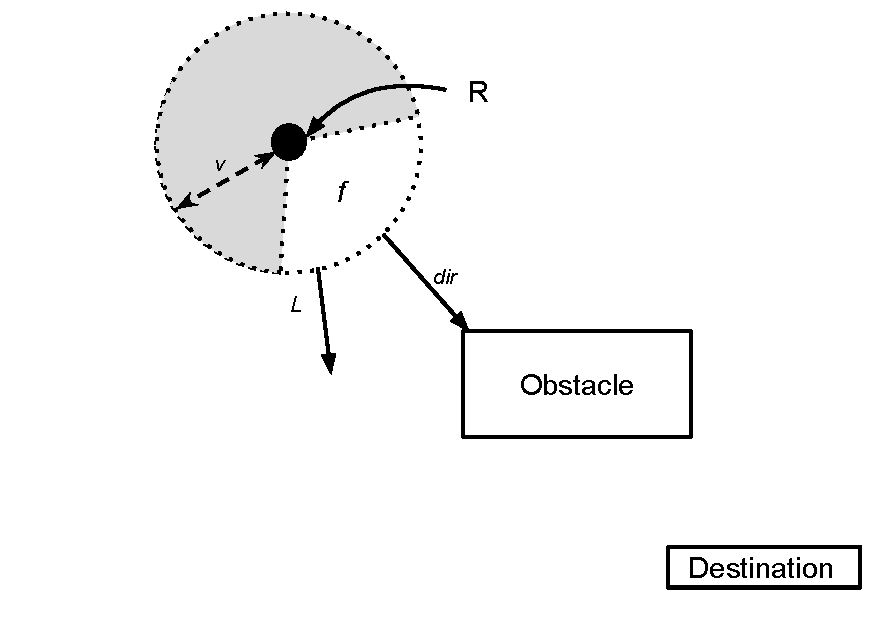
\includegraphics[width=0.75\textwidth]{chapters/chapter5/figures/ObstacleAvoidance.pdf}
	\caption{Navigation and Obstthe acle Avoidance, where $v$ is depth of view, $f$ is the field of view, $R$ is the robot, $dir$ is the direction of the destination and $L$ is a possible value of local attractor}
	\label{fig:obstacleavoidance}
\end{figure}


%%%%%%%%%%%%%%%%%%%%%%%%%%%%%%%%%%%%%%%%%%%%%%%%%
%%%%%%%%%%%%%%%%%%%%%%%%%%%%%%%%%%%%%%%%%%%%%%%%%
\section{Simulator}
\label{simulator}
A spatially discrete 2-dimensional grid world simulator has been developed and used in this thesis in order to accelerate computation \cite{sugawara2002swarming}. In real root experiments, algorithm performance is sensitive to the amount of time taken to load items and manoeuvre the robots \cite{ostergaard2001emergent}. The 2-dimensional grid world simulator allows for movement and loading time to be standardized across all algorithms for effective comparison.

The simulation robots function as follows:
\begin{itemize}
	\item Each robot fits into one grid block and each item takes up one grid block. 
	\item Only one item or robot can occupy a grid block at a time, which will allow for collisions and congestion to occur. 
	\item Each robot can move to an adjacent cell in any direction.
	\item Robots can load, transport and offload a single item at a time.
	\item If a robot does not pick up an item, the item forms an obstacle that must be navigated around.
\end{itemize}

The prioritized and non-prioritized sinks were placed next to each other, on a single side of the environment. The sinks were marked by light beacons that all robots can detect and navigate towards. The reason the sinks were not placed in the centre of the environment as is commonly found in swarm robotics research \cite{labella2006division} is because the original prioritized foraging problem was inspired by the use of robots to forage gold and waste in mining tunnels. A mining tunnel has a single entrance where the gold and waste must be moved to, in order to be transported to the surface \cite{brune2010extracting}. Since there is only a single entrance at the beginning of a tunnel, the sinks need to occur at the beginning of the tunnel so that the items can be easily exported.

\section{Environments}
\label{experimentenvironments}

The experiments are to be run in environments wit different item distributions, sizes, item densities and different ratios of prioritized to non-prioritized items. 

The sizes of the environment grid, $S$, were varied, where $S\in{50,100,200,300, 500}$, such that $S$ is the width and length of the grid.  Experiments were run on different environment size to test how an algorithm can scale to larger environments. Different values for The density of the items on the grid ,$p$, were chosen where $p\in{0.05$, $0.2$, $0.5$, $0.7$, $0.9}$. Environments with a higher item density are more complex too forage since there exists a higher probability of a non-prioritized blocking the path to prioritized items.

The ratio of prioritized to non-prioritized items $r$, was varied, where $r\in{0$, $0.2$,$0.25$, $0.333$, $0.5$, $0.667$, $0.75$, $0.8$, $1$} where 0 is where there are no prioritized items on the grid and 1 has only prioritized items on the grid.

In environments with a small $r$ value, the abundance of non-prioritized items increases the likelihood of non-prioritized items blocking the access to prioritized items. The value of $r$ was also varied to determine if the exists a relationship between values of $r$ and the values for the ratio of robots assigned to forage prioritized items, $\tau$, in terms of the parameters' effect on the performance of each algorithm. Finally, the value of $r$ is varied in order to determine if the algorithms can adapt the ratio of robots foraging prioritized items $\tau$ to optimally forage an environment of a given $r$. 

Different item distributions were chosen to examine different capabilities of the algorithms. The item distributions are shown in Figure~\ref{fig:environments}, where each lighter shaded square is a prioritized item. A non-prioritized item is shown by a darker shaded square. Four different classes of environments were randomly generated as follows:

\begin{enumerate}

\item Environments where positions for items of each priority are selected from a uniform distribution, refer to Fig~\ref{fig:uniformenv}. The uniformly distributed environment is used as a control environment to test the algorithms is that there is no spatial relationship relationship between items of the same type.

\item For the Gaussian environments, the positions of the prioritized items are sampled from a Gaussian distribution , where the mean is the centre of the grid, and the distribution varies, refer to Fig~\ref{fig:gaussianenv}. 

The positions of the non-prioritized items are selected after placing the prioritized items. The position for the non-prioritized items are selected from a uniform distribution. 

In Gaussian distribution environments, prioritized items occur much more frequently and tightly packed in the center of the environment. More non-prioritized items occur on the outskirts of the environment, surrounding the prioritized items in the centre.

The Gaussian environments were used to examine whether an algorithm can deal with foraging the non-prioritized items  or navigating past non-prioritized items to reach prioritized items. 


\item Environments with a clustered items disitrubtion  have clusters of items of the same type, refer to Fig~\ref{fig:clusterenv}. The clusters are generated by Lumer-Faieta ant cemetery clustering \cite{lumer1994diversity}. Each cluster is labelled randomly as a cluster of prioritized or non-prioritized items. 

The goal of performing experiments in a clustered environment was to test an algorithms ability to exploit areas which are rich in prioritized items. Clustered environments are also be used to test if an algorithm aids navigation around non-prioritized items. 

\item Environments with a vein distribution resemble the patterns observed in naturally occurring gold reefs \cite{frimmel2002recent}, refer to Fig~\ref{fig:veinenv}. In a gold reef, molten gold fills planar fractures between rock resulting in a vein of gold. Inspired by the gold reef, vein distributed environments have a long thin vein of prioritized items running form one side of the environment to another. The vein of prioritized items is surrounded by non-prioritized items. The non-prioritized items are similar to the rock surrounding the gold in gold reefs.

Experiments run in a vein environment aimed to test whether robots of a specific algorithm can follow and forage the continuous vein of prioritized items. A swarm that could detect the location of the vein and return to the vein's location after foraging an item should forage more than one that cannot detect and remember the location of the vein.

\end{enumerate} 

\vspace{-2em}
\begin{figure} [h]
        \centering
        \begin{subfigure}[b]{0.21\textwidth}
                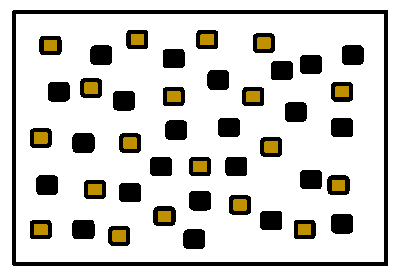
\includegraphics[width=\textwidth]{chapters/chapter4/figures/uniformenv.pdf}
                \caption{Uniform}
                \label{fig:uniformenv}
        \end{subfigure}%
        \begin{subfigure}[b]{0.205\textwidth}
                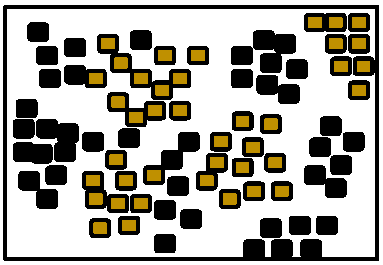
\includegraphics[width=\textwidth]{chapters/chapter4/figures/clusterenv.pdf}
                \caption{Clustered}
                \label{fig:clusterenv}
        \end{subfigure}
        \begin{subfigure}[b]{0.2\textwidth}
                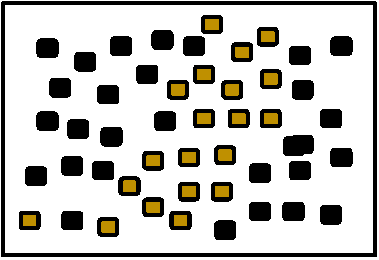
\includegraphics[width=\textwidth]{chapters/chapter4/figures/veinenv.pdf}
                \caption{Vein}
                \label{fig:veinenv}
        \end{subfigure}  
        \begin{subfigure}[b]{0.2\textwidth}
                        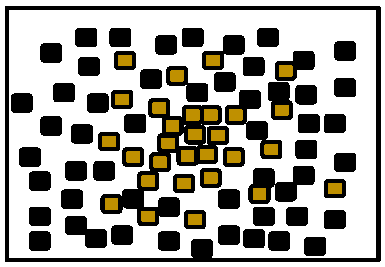
\includegraphics[width=\textwidth]{chapters/chapter4/figures/gaussianenv}
                        \caption{Gaussian}
                        \label{fig:gaussianenv}
       \end{subfigure}
        \caption{Environment Classes}\label{fig:environments}
\end{figure}


\section{Swarm Parameters}
\label{parameters}

For all algorithms, the robot swarm was initialized with 
a ratio of robots foraging prioritized items, $\tau$ versus non-prioritized items, where $\tau\in{0$, $0.2$, $0.25$, $0.333$, $0.5$, $0.667$, $0.75$, $0.8$,$1$} such that 0 is where no robots initially forage prioritized items and 1 is where all robots initially forage prioritized items. As discussed in Section~\ref{experimentenvironments}, $\tau$ is varied, along with $r$, to determine if the relationship between those parameters has an effect on algorithm performance. Also, the ability of an algorithm to adapt the value of $\tau$ appropriately for a given $r$, gives a measure for testing flexibility of the algorithms.

The density of robots, $c$, is defined as the density of cells of the grid size $S$ (the length of the side of an environment) that are occupied by robots, where $c=0.1, 0.3, 0.5, 0.7, 1$. The density of robots is varied in order to test the scalability of the algorithm. The density of robots is also varied to test an algorithms ability to adjust the amount of active foraging to the density of the items in the environment.

Honey bee specific parameters were selected based on \cite{seeley2009wisdom} as
-$t_{max}=200$ time steps, $f_{max}=100$ time steps, $\phi=0.8$ and $\rho=0.1$. Testing the effect of each of the honey bee algorithm specific parameters was not in the scope of this thesis.

The initial position of each robot was randomly selected, adjacent to the sink. All robots began in the exploration state, which a state that is shared by all algorithms. For each set of algorithmic, environmental and swarm configurations, each sample was run for 10000 time steps. An experiment consists of 30 repeated sample runs.

\section{Performance Measures}
\label{thri:third:performancemeasures}

%What do I need to add to 
%TODO: The idea is to add more robots foraging the prioritized items.
The following performance measures were used: 

	\begin{itemize}
		\item	The percentage of prioritized items foraged over time,  $\sigma$ 
		\item	The percentage of non-prioritized items foraged over time, $\mu$
		\item   The average time spent by agents waiting at the sink, $\epsilon$
	\end{itemize}
	
Future studies could include the average time taken by a robot to forage an item, the average distance moved by a robot and a measure to explain the randomness of a robots movement. 



%%%%%%%%%%%%%%%%%%%%%%%%%%%%%%%%%%%%%%%%%%%%%%%%%

%%%%%%%%%%%%%%%%%%%%%%%%%%%%%%%%%%%%%%%%%%%%%%%%%
%%%%%%%%%%%%%%%%%%%%%%%%%%%%%%%%%%%%%%%%%%%%%%%%%
%%%%%%%%%%%%%%%%%%%%%%%%%%%%%%%%%%%%%%%%%%%%%%%%%
%%%%%%%%%%%%%%%%%%%%%%%%%%%%%%%%%%%%%%%%%%%%%%%%%
\section{Summary}
\label{third:summary}
The robots used in this study are based on that of the e-puck robots, but with gripper capabilities. The robots used a navigation and obstacle avoidance technique based on the flocking behaviour of birds where a global attractor force attracts the robot in a specific direction, while the local attractor force guide the robot around localized obstacles. A simple 2-dimensional grid-based simulator is used. Only a single robot or item could occupy a single grid cell at once.

The environment types that were generated for experimentation in order to test different properties of the algorithms are discussed. The environment types defined have the four following distributions: uniform distribution, Gaussian distribution, clustered distribution and vein distribution. The following environmental parameters were varied: item density, environment size and item type ratio. The following swarm parameters chosen for each of the algorithms were presented: initial swarm configuration, swarm density, and honey bee specific parameters. Performance measures were selected to compare different aspects of the algorithms: the different percentages of each type of item foraged as well as the time spent waiting by the sink. 



%%%
%%%%%%%%%%%%%%%%%%%%%%%%%%%%%%%%%%%%%%%%%%%%%%%%%
%%%%%%%%%%%%%%%%%%%%%%%%%%%%%%%%%%%%%%%%%%%%%%%%%